\name{Diego Barquero Morera}
\address{Adresse : Île-de-France, Créteil, 5 Rue des Bordières}
\address{Téléphone (Costa Rica) : (+506) 8714 4835, Téléphone (France) : (+33) 745 105 417}
\address{Email : \href{mailto:diego.barqueromorera@studenti.unitn.it}{diego.barqueromorera@studenti.unitn.it} $\qquad$ \href{https://github.com/DiegoBarMor}{GitHub} $\qquad$ \href{https://www.linkedin.com/in/diego-barquero-morera-98863020b/}{LinkedIn}}
\begin{document}


%\scriptsize{\small}
%--------------------------------------------------------------------
%    SECTION ÉDUCATION
%--------------------------------------------------------------------

\begin{rSection}{Éducation}

    \vspace{\baselineskip}

    {\bf \href{https://u-paris.fr/en/}{Université Paris Cité (UPC), Paris, France}} \hfill {01.03.2023–31.10.2023} \\
    \textit{Stage}\\
    Intitulé du stage : "Caractérisation physique des sites de liaison protéine/ligands pour la visualisation en réalité augmentée"\\

    {\bf \href{https://www.unitn.it/}{Università degli Studi di Trento (Unitn), Trento, Italie}} \hfill {13.09.2021-14.12.2023} \\
    \textit{Master en Sciences quantitatives et informatiques}\\
    Intitulé de la thèse : "Caractérisation physique des sites de liaison des protéines et de l'ARN et leur représentation graphique dans le logiciel de visualisation moléculaire UnityMol"\\

    {\bf \href{https://www.tum.de/en/}{Technical University of Munich (TUM), Munich, Allemagne}}\hfill {01.04.2019-30.09.2019}\\
    \textit{Programme d'échange}\\
    Cours suivis à la Faculté de Chimie (Biologie moléculaire et Chimie organique)\\

    {\bf \href{https://www.tec.ac.cr/}{Institut de technologie du Costa Rica (TEC), Cartago, Costa Rica}} \hfill {08.02.2016-02.09.2021} \\
    \textit{B.Sc. en Génie biotechnologique}\\
    Intitulé de la thèse : "Proposition de comparaison des flux métaboliques en adaptant des algorithmes aux voies métaboliques"\\
    Note : 100/100 avec distinction


\end{rSection}
%--------------------------------------------------------------------
%    SECTION COMPÉTENCES TECHNIQUES
%--------------------------------------------------------------------

\begin{rSection}{Compétences}
    \vspace{\baselineskip}
    \subsection*{}

    %%%%%%%%%%%%%%%%%%%%%%%%%%%%%%%%%%%%%%%%%%%%%%%%%%%%%%%%%%%%%%%%%%%%%%%%%%%%%%
    \begin{table}[h!]
        \centering
        \captionof*{table}{Langages informatiques}
        \begin{tabular}{llll}
            %%%%%%%%%%%%%%%%%%%%%%%%%%%%%%%%%%%%
            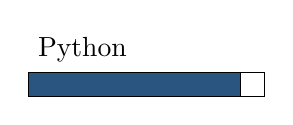
\begin{tikzpicture}
                \node [anchor=west] at (0,.6) {Python};
                \draw [fill=white] (0,0) rectangle (3,.3);
                \draw [fill={rgb:red,1;green,2;blue,3}] (0,0) rectangle (2.7,.3); %90%
            \end{tikzpicture} &

            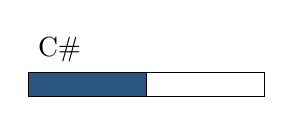
\begin{tikzpicture}
                \node [anchor=west] at (0,.6) {C\#};
                \draw [fill=white] (0,0) rectangle (3,.3);
                \draw [fill={rgb:red,1;green,2;blue,3}] (0,0) rectangle (1.5,.3); %50%
            \end{tikzpicture} &

            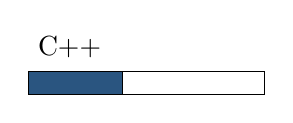
\begin{tikzpicture}
                \node [anchor=west] at (0,.6) {C++};
                \draw [fill=white] (0,0) rectangle (3,.3);
                \draw [fill={rgb:red,1;green,2;blue,3}] (0,0) rectangle (1.2,.3); %40%
            \end{tikzpicture} &

            
\begin{tikzpicture}
                \node [anchor=west] at (0,.6) {JavaScript, Java};
                \draw [fill=white] (0,0) rectangle (3,.3);
                \draw [fill={rgb:red,1;green,2;blue,3}] (0,0) rectangle (0.75,.3); %25%
            \end{tikzpicture} \\

            %%%%%%%%%%%%%%%%%%%%%%%%%%%%%%%%%%%%
            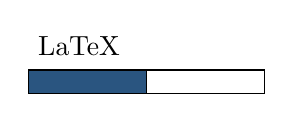
\begin{tikzpicture}
                \node [anchor=west] at (0,.6) {LaTeX};
                \draw [fill=white] (0,0) rectangle (3,.3);
                \draw [fill={rgb:red,1;green,2;blue,3}] (0,0) rectangle (1.5,.3); %50%
            \end{tikzpicture} &

            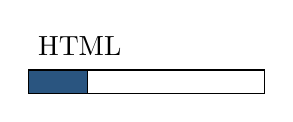
\begin{tikzpicture}
                \node [anchor=west] at (0,.6) {HTML};
                \draw [fill=white] (0,0) rectangle (3,.3);
                \draw [fill={rgb:red,1;green,2;blue,3}] (0,0) rectangle (.75,.3); %25%
            \end{tikzpicture} &

            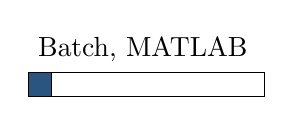
\begin{tikzpicture}
                \node [anchor=west] at (0,.6) {Batch, MATLAB};
                \draw [fill=white] (0,0) rectangle (3,.3);
                \draw [fill={rgb:red,1;green,2;blue,3}] (0,0) rectangle (.3,.3); %10%
            \end{tikzpicture} &

        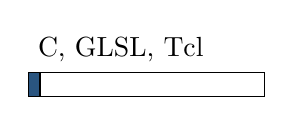
\begin{tikzpicture}
            \node [anchor=west] at (0,.6) {C, GLSL, Tcl};
            \draw [fill=white] (0,0) rectangle (3,.3);
            \draw [fill={rgb:red,1;green,2;blue,3}] (0,0) rectangle (.15,.3); %5%
        \end{tikzpicture}

        %%%%%%%%%%%%%%%%%%%%%%%%%%%%%%%%%%%%
        \end{tabular}
        \caption*{Expérience en utilisant les environnements de développement Unity3D (C\#), Android Studio (Java) et Visual Studio (C++/C\#).}
\end{table}


%%%%%%%%%%%%%%%%%%%%%%%%%%%%%%%%%%%%%%%%%%%%%%%%%%%%%%%%%%%%%%%%%%%%%%%%%%%%%%
\begin{table}[h!]
\centering
\captionof*{table}{Langues étrangères}
\begin{tabular}{llll}
    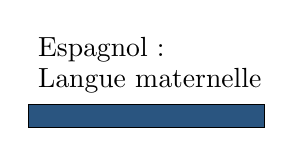
\begin{tikzpicture}
        \node [anchor=west] at (0,1.) {Espagnol :};
    \node [anchor=west] at (0,.6) {Langue maternelle};
        \draw [fill=white] (0,0) rectangle (3,.3);
        \draw [fill={rgb:red,1;green,2;blue,3}] (0,0) rectangle (3,.3);
    \end{tikzpicture} &

    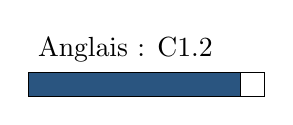
\begin{tikzpicture}
        \node [anchor=west] at (0,.6) {Anglais : C1.2};
        \draw [fill=white] (0,0) rectangle (3,.3);
        \draw [fill={rgb:red,1;green,2;blue,3}] (0,0) rectangle (2.7,.3);
    \end{tikzpicture} &

    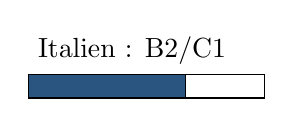
\begin{tikzpicture}
        \node [anchor=west] at (0,.6) {Italien : B2/C1};
        \draw [fill=white] (0,0) rectangle (3,.3);
        \draw [fill={rgb:red,1;green,2;blue,3}] (0,0) rectangle (2,.3);
    \end{tikzpicture} &

    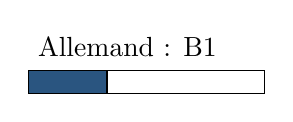
\begin{tikzpicture}
        \node [anchor=west] at (0,.6) {Allemand : B1};
        \draw [fill=white] (0,0) rectangle (3,.3);
        \draw [fill={rgb:red,1;green,2;blue,3}] (0,0) rectangle (1,.3);
    \end{tikzpicture}
\end{tabular}
\end{table}


\end{rSection}

\vspace{\baselineskip}
\begin{flushright} \small{Mise à jour : \today} \end{flushright}


\end{document}
